%----------------------------------------------------------------------------
\chapter{Financial frauds}
%----------------------------------------------------------------------------

In today's world, most of the purchases are made electronically. 
Instead of cash, we use bank cards in shopping with point of sale (POS) or provide our card details, even in the most basic web shopping sites.
While internet is open for anyone, the vulnerability can be misused by other people.
In a basic scenario, data breaches give fraudsters our sensitive data to use in fake financial transactions.
The continually increasing number of fraud records pushes financial institutions to develop fraud detection and prevention systems.

%----------------------------------------------------------------------------
\section{Fraud detection methods}
%----------------------------------------------------------------------------

One of the methods used today to detect fraudulent transactions is a historical record based machine learning.
In this method, the system is trained by processed historical transaction datasets, where fraudulent records have been labelled.
To improve the learning process, experts also add their own rules.
These rules can be constrained with payment location, time of day, cardholder gender specification, and more.

In the optimistic case, the fraudulent transaction is detected simultaneously, and preventive actions will be taken.
In the case of bypassed fake transactions, it is more likely to be repeated until the card owner blocks it.
The transaction pattern of hacked accounts by post-processing is valuable input for future rule-based machine learning systems.

The historical data based learning systems require human experts for calibration.
The participation of humans has advantages to define more special scenario rules or to correct legit transactions that have been marked false alarm by the system alone.
From the other perspective, machine learning algorithms can extract the hidden parameters that have to affect a fraudulent transaction, which is hard to detect by humans.

The database topology of the system is as important as data processing algorithms.
Each entry in the database has its own load on query execution.
Graph database topology is widely used to meet the reactive response behavior in transaction processing applications nowadays.
In a big scale picture, the density of the connection between data entries gives a more intuitive understanding of the system.
As discussed, the importance of human interaction with machine learning systems, graph database give people access to design query in an understandable rational way and faster.
This is why fraud detection is among the three most popular graph database applications~\cite{DBLP:journals/pvldb/SahuMSLO17}.

The main advantage of graph processing systems is the ability to find cyclic patterns considerably faster than relational databases.
Especially in financial fraud cases, cyclic patterns are commonly under investigation; these transactions cause fraudsters to perform illegal actions much cheaper than it would otherwise be possible.
For example, in e-commerce web sites, one fraud case is described as a merchant receives purchases from several accounts; those owners are also in the friendship cycle of the merchant.
With these transactions, merchants increase their ratings and mislead future customer decisions.
In another example, ``criminal'' customers using fake ID tries to purchase the partner merchant with short term credit from the bank. 
As a merchant receives the payment by bank transfers, the amount is transferred to the ``criminal'' via the middleman account.
To detect this kind of cyclic fraud transaction series in real time, a graph database engine (TigerGraph) was utilized in the Alibaba web platform~\cite{DBLP:journals/pvldb/QiuCQPZLZ18}.
In another example, suspicious payment patterns are trying to be revealed by finding fully connected subgraphs, and bicliques~\cite{DBLP:conf/ieaaie/BraunCSKL17}.

%----------------------------------------------------------------------------
\section{Fraud scenarios}
%----------------------------------------------------------------------------

A common of criminals with a significant amount of cash is hide it from legal authorities and move it without getting noticed.
As they often cannot transfer money in cash with suitcases, online transaction systems became their new target.
They used several innovative methods to ``launder'' money through bank systems, cover the transactions with legitimate enterprise reasons.
As financial institutions try to define new rules in fraud detection systems, the process is getting more complex over time.
Three of the recently popular fraud scenarios will be discussed and analyzed in this work.

\paragraph{Smurfing}

To avoid the banks' alert flags, criminals transfer their large amount with small, distributed pieces called ``smurfs''.
In the U.S., banks are obliged to give a governmental report for each person who made a transaction over \$10\ 000.
So fraudsters always do their business under this limit.
Students are commonly targeted for this method, and they asked to retransfer the receiving amount for \$10--20 earnings.
Banks have monitored the customers continuously raising red flags for authorities if they have reliable facts.
However, false alarms can also be problematic and results in fines~\cite{Bloomberg19}.
In this situation, banks are complaining about rules that make them care and monitor customers, incurring significant extra costs.
The middlemen players depicted in \autoref{fig:smurfing} are involved in retransferring the amount they received from the ``Sender'' to the ``Receiver''.

\begin{figure}[!ht]
    \centering
    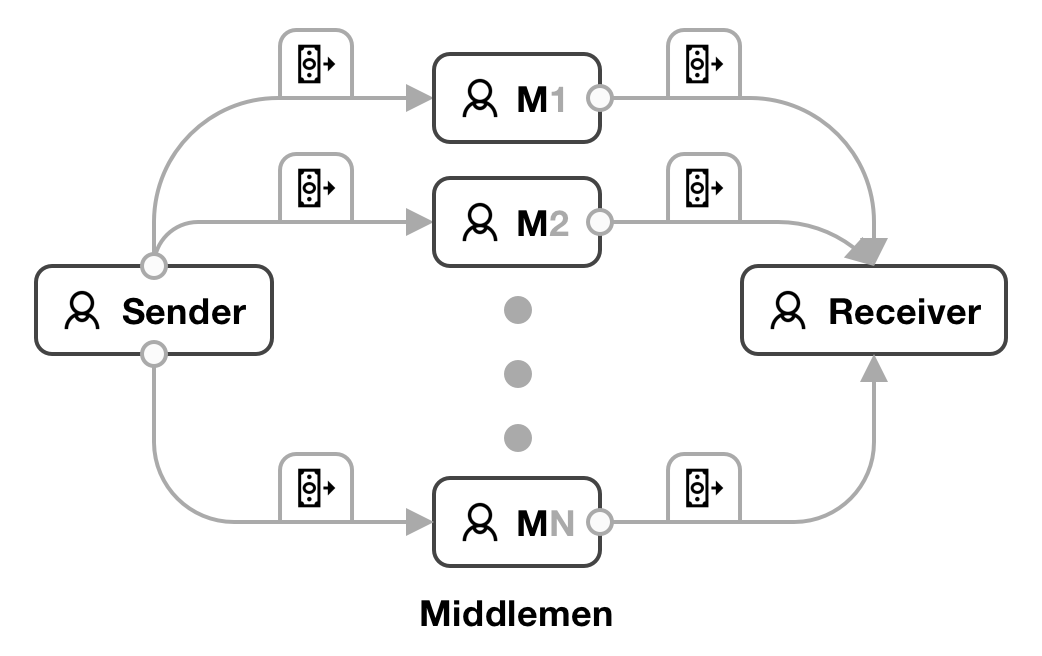
\includegraphics[scale=0.3]{figures/smurfing.png}
    \caption{Smurfing fraud scenario} 
    \label{fig:smurfing}
\end{figure}

\paragraph{Money laundering cycle}

As discussed before, it is common in e-commerce platforms to use cyclic transactions in order to get the desired rating or statistics.
With growing mobile banking providers, ``criminals'' found a new way to ``launder'' their money with a simpler method.
To make the transactions seem blurry, several middlemen involved in their cyclic transactions as shown in \autoref{fig:mobile_banking}.
It is still challenging to find a connection between initial sender and receiver in traditional banking systems, but today's mobile banking databases have connection maps~\cite{EIFREM20196}.
Through these databases, we can determine the close friendship connections between two customers and reactively detect such a fraudulent pattern.
In our implementation, several middleman people participate in cyclic paths.

\begin{figure}[!ht]
    \centering
    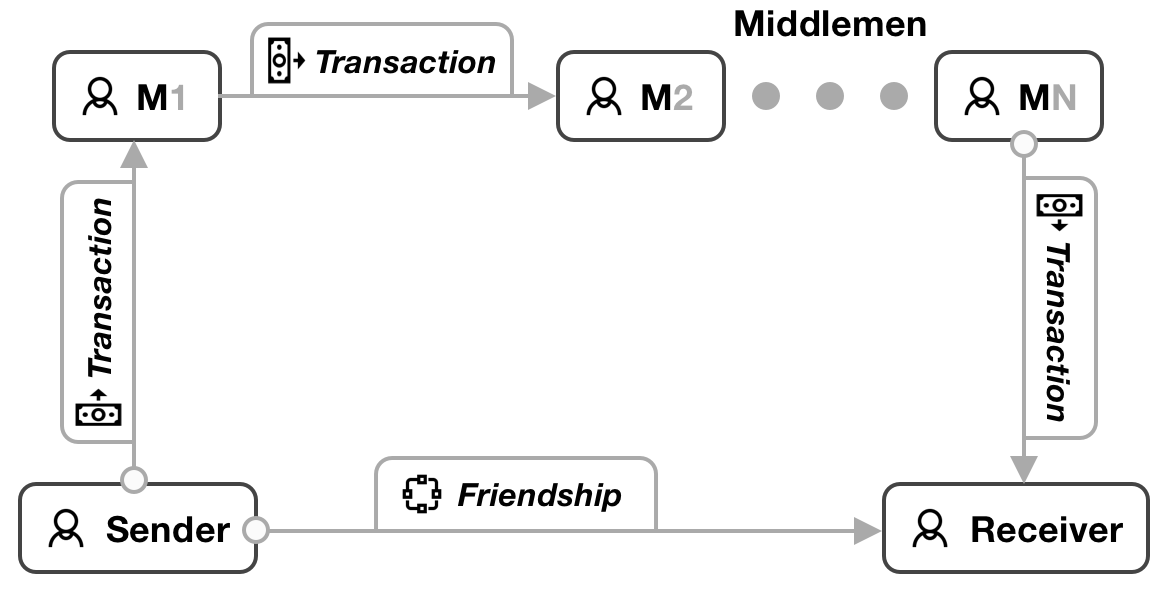
\includegraphics[scale=0.3]{figures/mobile_banking.png}
    \caption{Money laundering cycle scenario}
    \label{fig:mobile_banking}
\end{figure}

\paragraph{Biased reviews in e-commerce}

One more interesting fraud case is happening in e-commerce platforms very often nowadays.
Merchants communicate with real users via several channels and offer them free goods for a 5-star rating deal.
With successful deals, merchants gain a good reputation in the platform with fake reviews and are likely to reach more customers.
This method can be considered as an exciting and useful marketing approach if they allow all ratings from customers.
In contrast, they resist customers from writing negative feedback, which becomes an unfair behavior for the community.
In our implementation, we will found customers with 5-star reviews as in \autoref{fig:biased_reviews}, who interact only with the specific merchant's goods.

\begin{figure}[!ht]
    \centering
    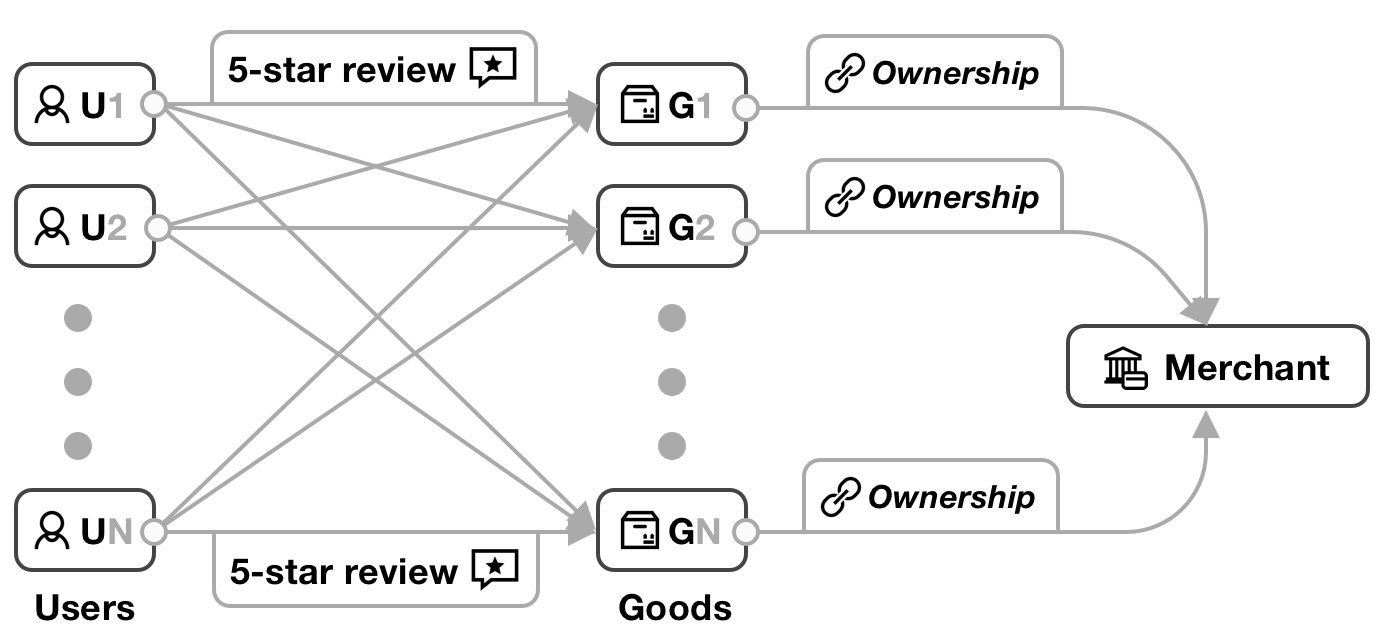
\includegraphics[scale=0.3]{figures/biased_reviews.png}
    \caption{Biased reviews in e-commerce scenario}
    \label{fig:biased_reviews}
\end{figure}
